\nextpage
\section{Опыт Б. Два представления переходов}
У собственных вариантов общий граф и один шаблон \code{next}. Одно и то же число $c(a)$ обозначает класс входного байта $a$. В варианте table новое состояние равно элементу $D[q,c(a)]$, в branch~--- значению, которое выбирает вложенное ветвление по $q$ и $c(a)$. Генератор построил обе записи из одного описания. Тест перебрал 61 состояние и все 256 значений байта. Для всех $61\cdot256=15\,616$ пар значения совпали. Следовательно, одинаковое начальное состояние даёт одинаковый путь по любому слову. Метки заключительных состояний и правило выдачи тоже общие.

Классификатор объединяет байты с одинаковыми переходами из всех состояний в 36 классов и занимает 256 байт. Для table массив переходов занимает ещё $61\cdot36=2\,196$ байт. В branch этот шаг выражен операторами \code{switch}. Независимый процедурный сканер подтвердил выдачу собственных вариантов на 81\,685 проверочных входах.

Для каждого входа и раунда $r$ взяты два времени из опыта~А:
\[
            R_r=T_{\mathrm{table},r}/T_{\mathrm{branch},r}.
\]
При $R_r>1$ быстрее branch, при $R_r<1$ быстрее table. Квартили вычислены после образования 16 пар.

\begin{center}
\captionof{table}{Парное отношение времён на тех же входах, что в таблице~\ref{tab:a}. Последний столбец показывает число раундов из 16, в которых быстрее branch. Значения $R$ безразмерны.}\label{tab:b}
\small\setlength{\tabcolsep}{5pt}\renewcommand{\arraystretch}{1.04}
\begin{tabular*}{.95\linewidth}{@{\extracolsep{\fill}}lrrrr@{}}
\toprule Вход & Медиана $R$ & $Q_1$ & $Q_3$ & Побед branch\\ \midrule
\rowsB
\bottomrule
\end{tabular*}
\end{center}

\nextpage
\section*{Где выгодны таблица и ветвления}
На учебном корпусе медиана $R$ равна 1,046, а средняя половина парных отношений лежит между 1,023 и 1,066. В 13 из 16 раундов branch закончил проход раньше. Направление большинства пар видно и при частичном перекрытии интервалов отдельных реализаций в опыте~А. Выигрыш на корпусе скромнее, чем на длинных однородных словах.

\begin{center}
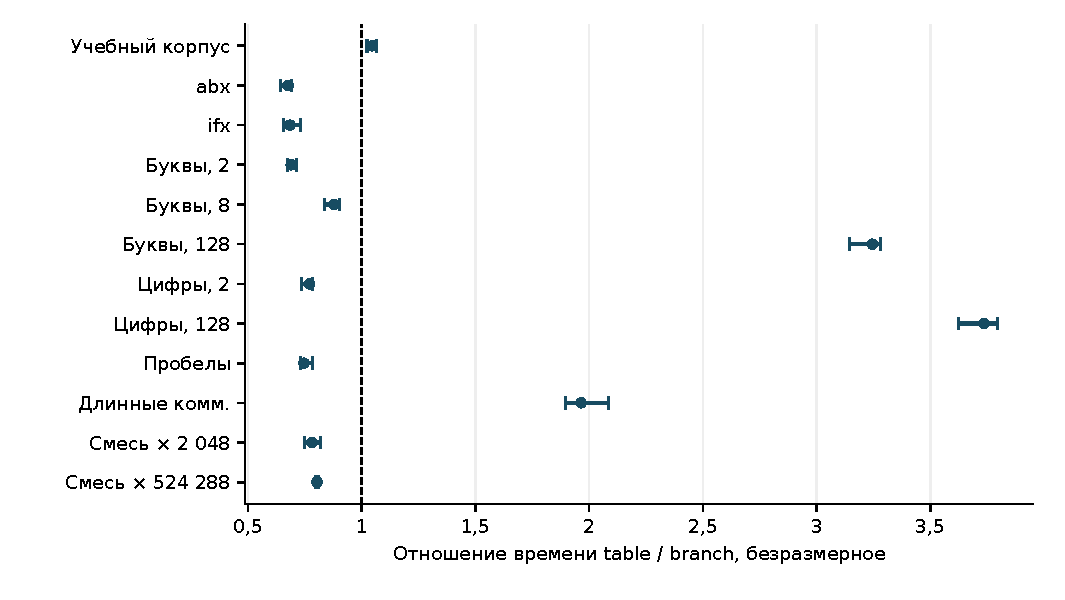
\includegraphics[width=.96\linewidth]{figures/ratios.pdf}
\captionof{figure}{Выбранные входы из таблицы~\ref{tab:b}. Точка~--- медиана парных отношений, горизонтальный отрезок~--- $[Q_1;Q_3]$. Штриховая вертикаль соответствует равному времени. Слева быстрее table, справа быстрее branch.}\label{fig:ratios}
\end{center}

\subhead{Что даёт общее начало с ключевым словом}
При замене всех \code{abx} на \code{ifx} медиана $R$ меняется с 0,677 до 0,685. Как и на смеси этих слов, во всех 16 парах выигрывает table. Для шестибайтовых слов переход от \code{abcde2} к \code{while2} приближает отношение к единице (с 0,803 до 0,932). Длина и выдача сохранены, но слово \code{while2} проводит автомат через состояния префикса ключевого слова. Влияние этого изменения зависит от выбранной пары.

\subhead{Одинаковое число имён, разное устройство пропусков}
На коротких комментариях $R=0,779$, на длинных $R=1,965$. В обоих случаях одинаковы объём входа, число имён и суммарный размер комментариев. В первом случае сканер часто входит в состояние комментария и покидает его. Во втором он дольше остаётся в этом состоянии. Направление преимущества изменилось во всех 16 парах. Чтобы отделить влияние ветвлений процессора от обращений к памяти, понадобились бы отдельные измерения.
